\subsection{Solutions Ideas:}

\begin{itemize}
\setlength{\itemsep}{0mm}
	\item Choose the ROI with user-input.
	\item Search for the table as the biggest contour.
	\item Searching for the pockets on the pool table.
	\item Finding the diamonds and using these to determine the ROI.
	\item Finding the most common colour (the cloth) and then find the outer points of the cloth.
\end{itemize}

\textbf{Choose The ROI With User-Input:}\\
This method would not require any image processing, but would require the user to set the ROI. This solution could be used if the chosen solution does not return a ROI due to difficult illumination or errors.

\textbf{Search For The Table As The Biggest Contour:}\\
The method was tried and gave mixed results. It was possible to segment the table using adaptive threshold and thereafter process it with OpenCV \cite{opencv} contour finding algorithm. This would find the outside of the table, but sometimes also the floor or anything underlying the table that was a bigger rectangle. \\

\textbf{Searching For The Pockets On The Pool Table:}\\
This proved to be easy to do by using the value part of the image in HSB colour space. Since the pockets are less illuminated than the rest of the table this should have a very low value. An example of this can be seen in\ref{fig:value_thres}. 

\begin{figure}[H]
\begin{center}
\leavevmode
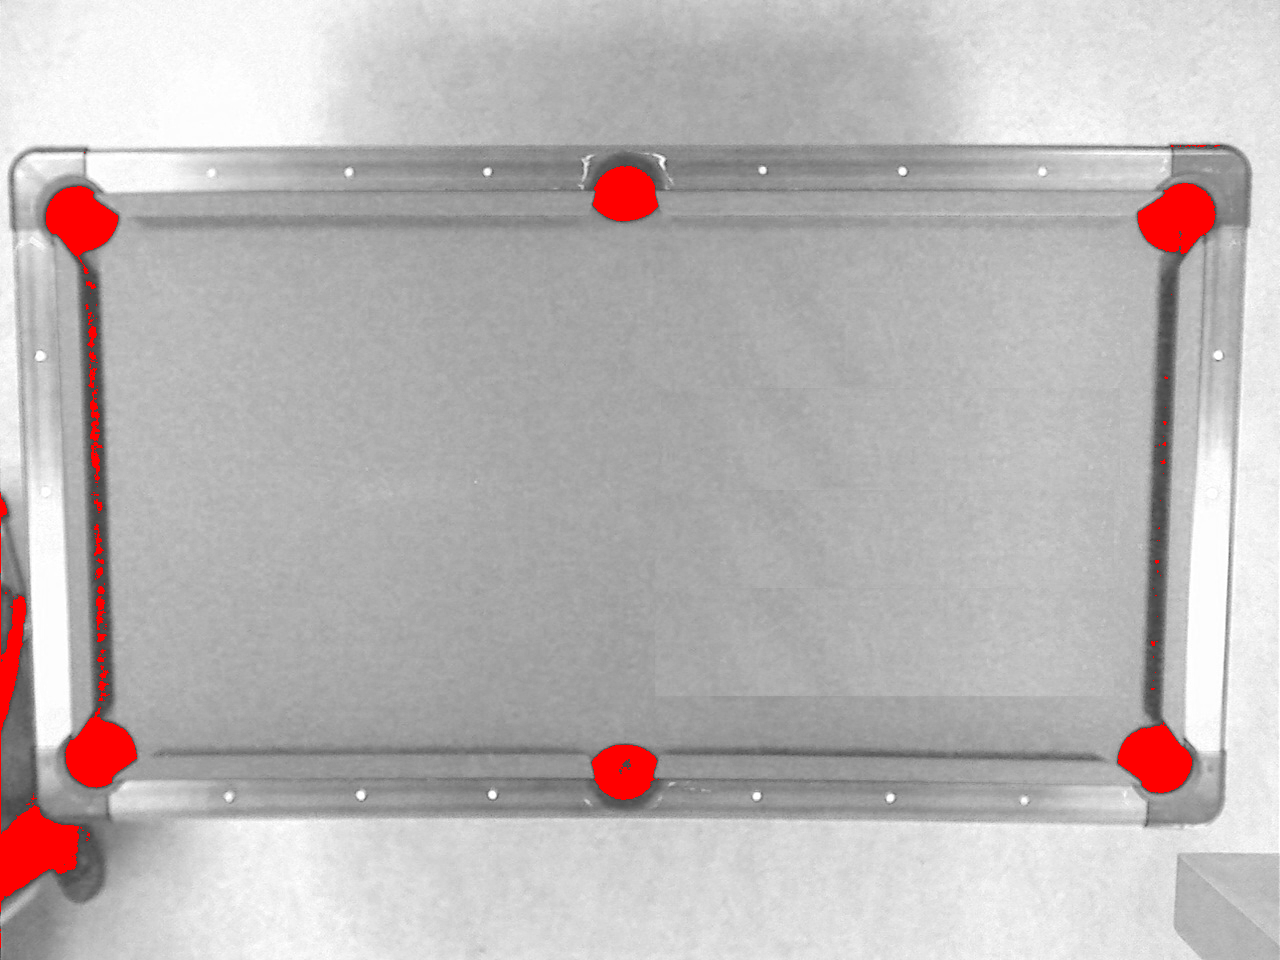
\includegraphics[width=0.5\textwidth]{images/value_thres}
\end{center}
\caption{Value part of HSB image thresholded.}
\label{fig:value_thres}
\end{figure}

As seen in\ref{fig:value_thres} a leg is also selected as a part of the outcome of the threshold. Several tried showed that the method was not quite robust enough for further use.\\

\textbf{Finding The Diamonds and Use These To Determine The ROI:}\\
Much time was used with this approach. The idea was to find the diamonds and the use these to find the exact ROI. The specifications \ref{sec:rules} of a regulation size pool table states that a diamond has to be 93.5 mm from the nose of the cushion. By finding the length between each diamond, which was also strictly specified, it would be possible to find a pixel-to-meter ration and thereby finding the precise ROI.\\

Some progress was made, but eventually this method was abandoned due to the fact that many of the pool tables, including the one where pictures for this  project was taken, did not follow these regulations. The idea was also to use the distance between diamonds to determine the exact size of a ball. Another approach for this will have to be used.\\

\subsection{Chosen Solution:}

\textbf{Finding The Most Common Color (The Cloth) And Then Find The Outer Points Of The Cloth.}\\
This solution showed to be the most robust since the cloth will take up at least 50\% and probably more of the entire image. This makes it a prime candidate for detecting. Also even in the odd coincidence where the colour of the floor and cloth are alike, the rails of the table will separate these and thereby still make it possible to detect the cloth.\\

As written in the pool table regulations \ref{sec:rules} the table has to be one of three colours: yellow-green, blue-green or electric blue. Different from the last method this seems to be the case for every pool table. That they have a solid colour which stands out.\\

This fact will be used as part of the solution for this problem. As shown on histograms in \ref{sec:analysisballstable} the hue part of the HSB colour space will to be good for separating the cloth from the rails and surroundings. Hue also has the useful property of, in theory, indifferent to illumination which should make it more robust for this solution. A flowchart of the solution can be seen in \ref{fig:tabledetect_flowchart}

%INDSÆT HISTOGRAM m. HUE over de fire forskellige billeder.

%The solution consists of the following steps:
%\begin{enumerate}
%\setlength{\itemsep}{0mm}
%	\item Convert the input image to HSB and make a new image for the hue.
%	\item Make a histogram of the value in the hue image.
%	\item Identify the pixels close to the maximum value of the hue histogram.
%	\item Remove noise by using a median filter.
%	\item Find the bounding box of the cloth and make a binary mask.
%	\item Find the angle of the cloth (and thereby table).
%	\item Output the ROI, angle and mask.
%\end{enumerate}

\begin{figure}[H]
\begin{center}
\leavevmode
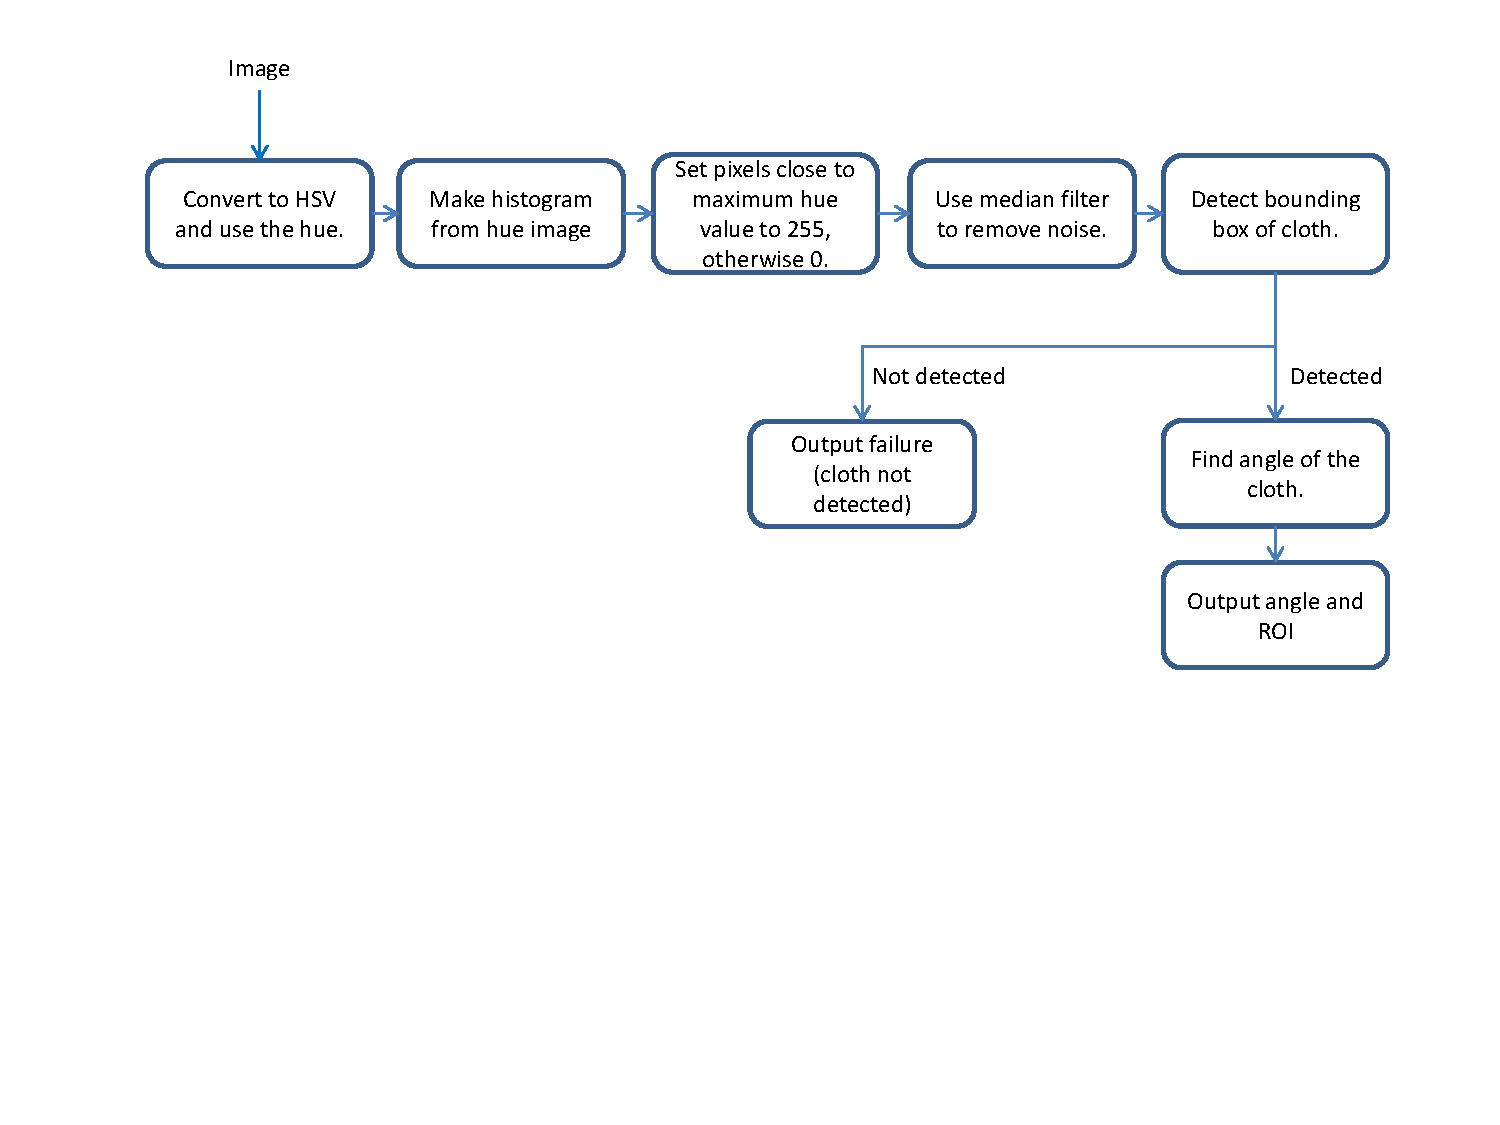
\includegraphics[width=0.8\textwidth]{images/tabledetect_flowchart}
\end{center}
\caption{Flowchart of the chosen solution}
\label{fig:tabledetect_flowchart}
\end{figure}

\subsubsection{The Solution In Details:}
\textbf{1) Convert The Input Image to HSB and Make A New Image For The Hue:}\\
This is done using the build in functions of OpenCV\cite{opencv}\fxnote{Necessary to cite them every time?}.\\

\textbf{2) Making The Histogram:}\\
Using the class DenseHistogram in OpenCV\cite{opencv} the histogram is computed from the hue image. A range of 0-255 is chosen together with 255 bins.\\

\textbf{3) Identify The pixels close To The Maximum Value Of The Hue Histogram.}\\
After finding the bin with the maximum value an iteration of the whole image is done to identify pixels close to the maximum value. The pixels that lie close are set to 255 (white) and the others are set as 0 (black). A threshold of $\pm$ 20 is set based on different tries. Since the illumination of the cloth is not exactly the same this value have to be higher than first expected.\\

The image after the cloth identification can be seen in \ref{fig:aftercloth}.

\begin{figure}[H]
\begin{center}
\leavevmode
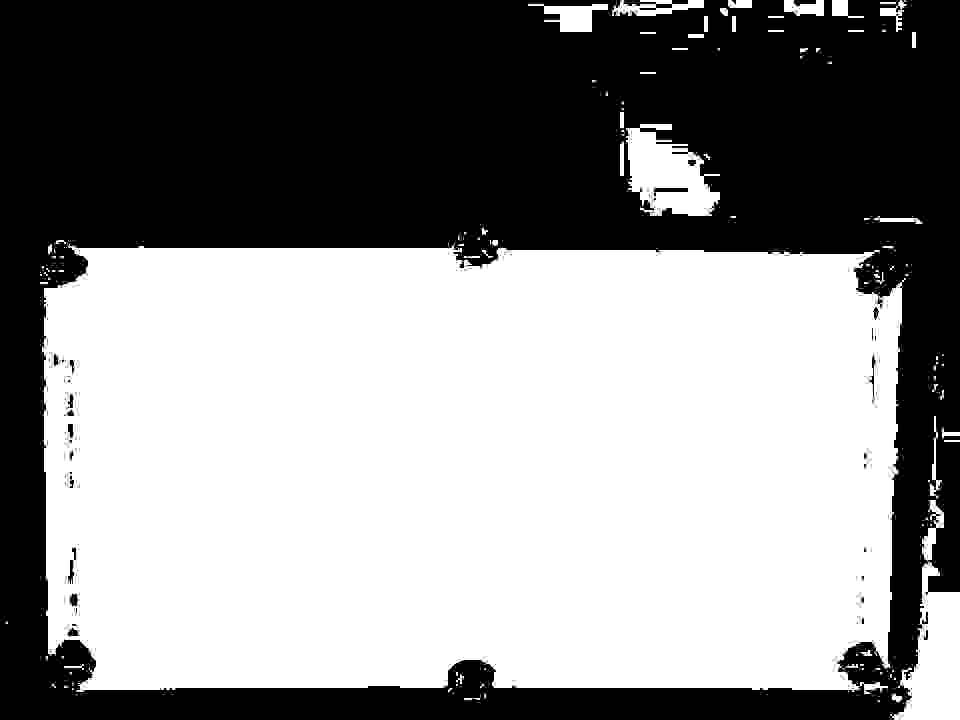
\includegraphics[width=0.5\textwidth]{images/aftercloth}
\end{center}
\caption{Image after cloth identification.}
\label{fig:aftercloth}
\end{figure}

\textbf{4) Remove Noise By Using A Median Filter:}\\
To remove noise from the image a median filter will be used. This allows the contour identifier in OpenCV\cite{opencv} to work optimal. If the median filter was not used potential contours could be much bigger than the cloth since one-pixel edges could connect across the rails from the cloth to floor. The outcome of the median filter can be seen in\ref{fig:afterclothmedian}

\begin{figure}[H]
\begin{center}
\leavevmode
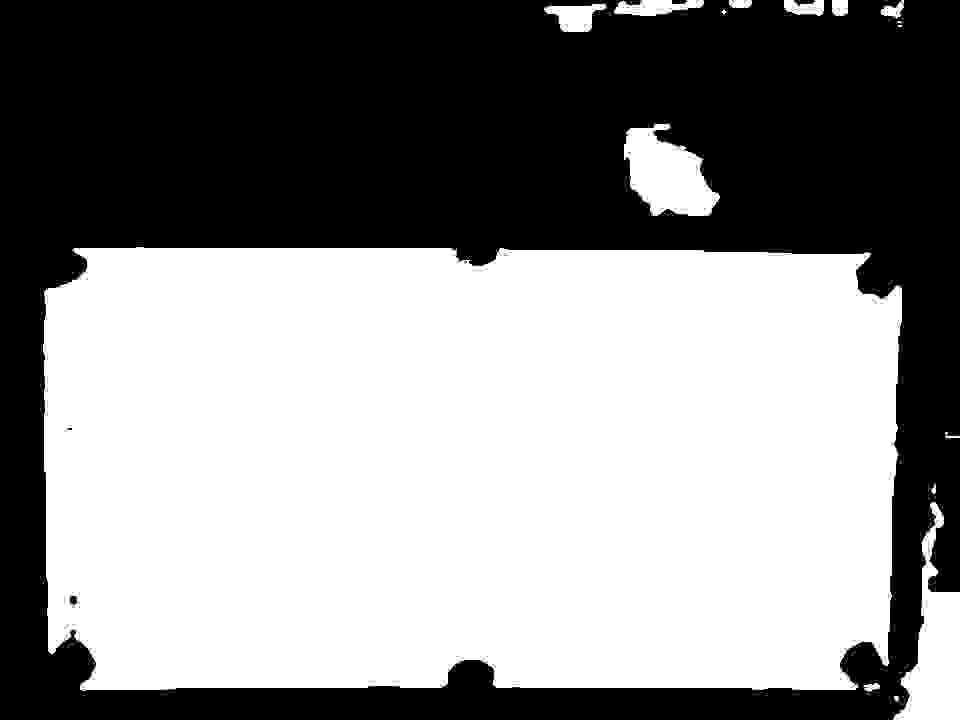
\includegraphics[width=0.5\textwidth]{images/afterclothmedian}
\end{center}
\caption{Image after median filter, kernelsize = 3.}
\label{fig:afterclothmedian}
\end{figure}

\textbf{5) Find The Bounding Box Of The Cloth and Make A Binary Mask:}\\
The cloth now appears as the biggest BLOB in the image. To find the bounding box of the cloth OpenCVs \cite{opencv} FindContours function is used. It uses the metod Suzuki85 developed by S. Suzuki and K. Abe \cite{contour}. The code iterates through the different contours found by FindContours. These contours are tested whether they could be the cloth by using a few conditions:

\begin{itemize}
\setlength{\itemsep}{0mm}
	\item The table is, as written in the requirements specification \ref{sec:reqspec}, required to take up at least 75\% of the frame area. Since the rails of the table is not detected the condition is set to the contour area having to be at least 50\% of the frame area. 
	\item Since the FindContours function sometimes identifies the entire image as a contour, the detected contour have an area smaller than the area of the image.
\end{itemize}

All the found contours can be seen in \ref{fig:allcontours}.
\begin{figure}[H]
\begin{center}
\leavevmode
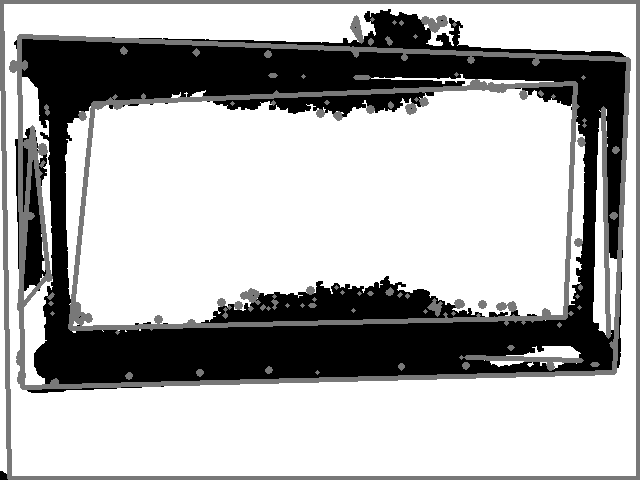
\includegraphics[width=0.5\textwidth]{images/allcontours}
\end{center}
\caption{All the contours found by FindContours after cloth identificationa and median filter.}
\label{fig:allcontours}
\end{figure}

The contour that is the output of the code above can be seen in \ref{fig:clothcontour}.
\begin{figure}[H]
\begin{center}
\leavevmode
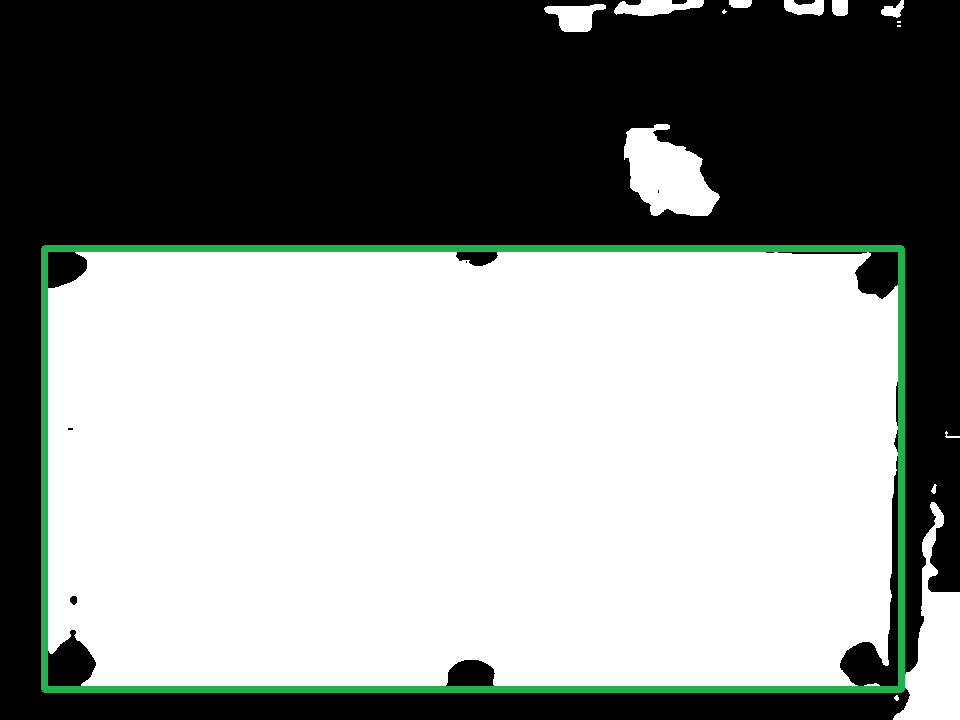
\includegraphics[width=0.5\textwidth]{images/clothcontour}
\end{center}
\caption{Cloth contour found by FindContours after cloth identificationa and median filter.}
\label{fig:clothcontour}
\end{figure}

A mask of the found contours is made. Since the box of the contour has to have straight edges this will be used to remove rails and pockets that could be in the image so this is not used when having to find the balls.

\begin{figure}[H]
\centering
\subfloat[Mask of cloth and other contours.]
{
	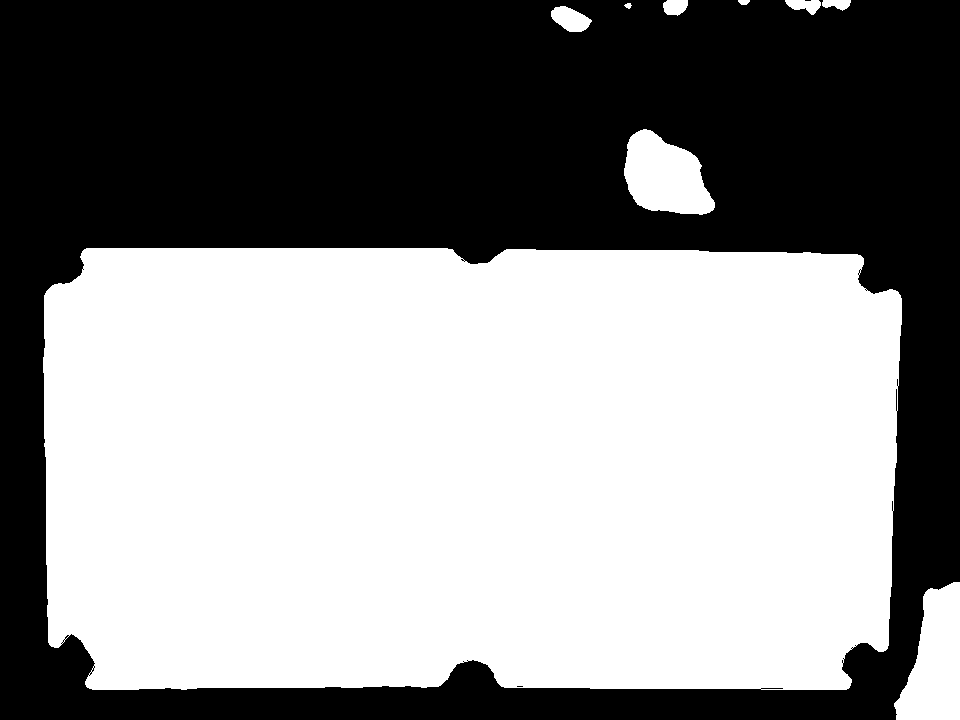
\includegraphics[width=0.3\textwidth]{images/mask_1}
}
\subfloat[Found contour of cloth.]
{
	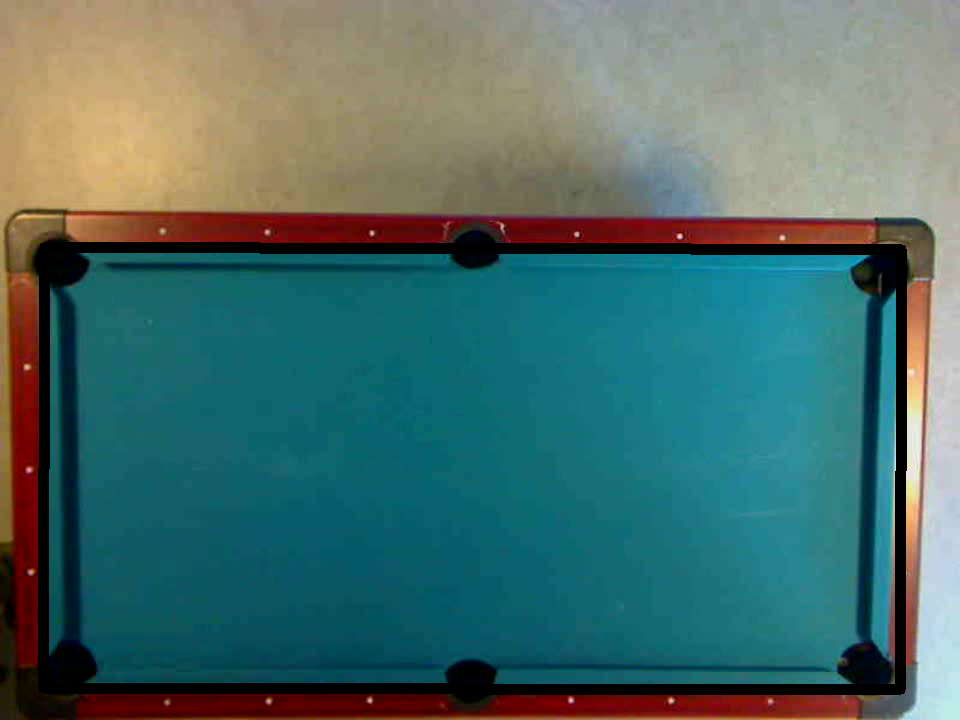
\includegraphics[width=0.3\textwidth]{images/mask_2}
}
\end{figure}

\textbf{6) Find The Angle Of The Cloth (And Thereby Table):}\\
To find the angle of the table the bounding rectangle of the contour of the cloth is divided into lines. A sort of the length is made and the longest line is selected. This line will always be the longest side of the table, the side that should be rotated to 0\degree. \\

The angle between the line and a horizontal line is calculated using the GetExteriorAngleDegree function in OpenCV\cite{opencv}. The angle found led to understand that there is a slight problem with the output as shown in \ref{fig:table_angle}.

\begin{figure}[H]
\begin{center}
\leavevmode
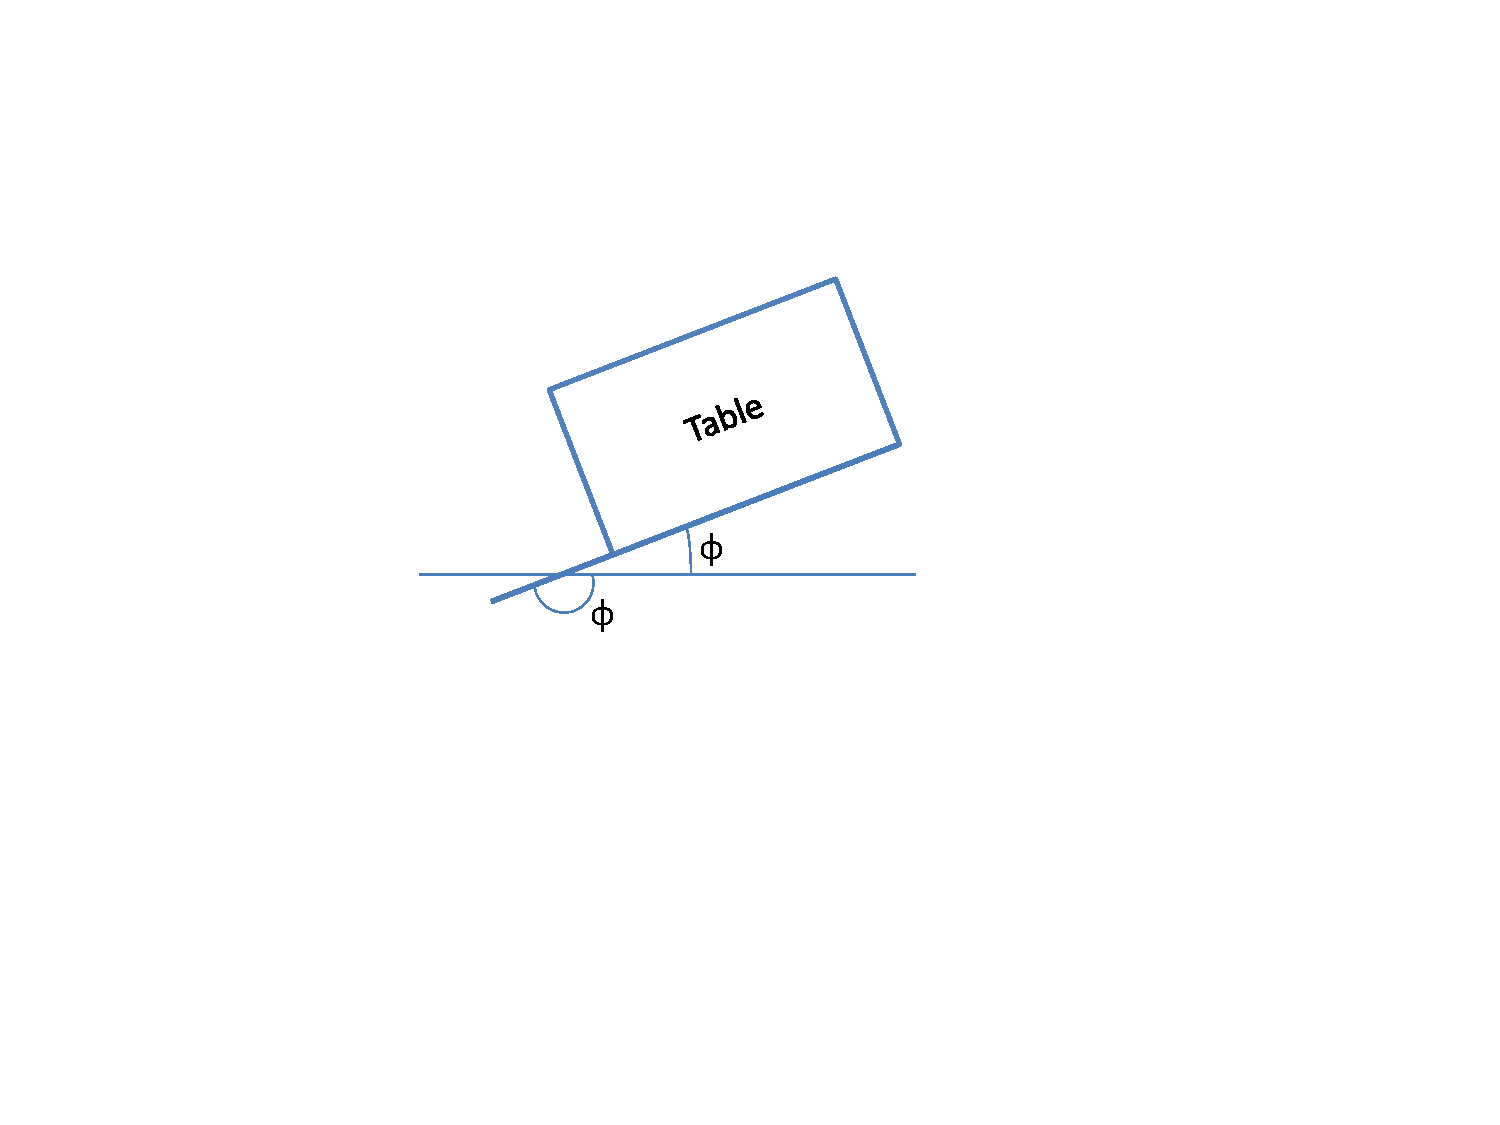
\includegraphics[width=0.5\textwidth]{images/table_angle}
\end{center}
\caption{The angle found between horizontal line and edge of table.}
\label{fig:table_angle}
\end{figure}

Therefore the if the angle is more than 90\degree is it calculated as angle = 180\degree-angle.\\

\textbf{7) Output The ROI, Angle and Mask:}\\
The angle and the box for the non-rotated image has been calculated. Since the calibration is not a time-critical part of the solution the ROI is found simply by rotating the image and running step 5 again.  This will rotate the image and then search for the ROI of the rotated image. A faster method would be calculating the new position of the ROI based on the rotated angle.
\\\\
The output can be seen in figure \ref{fig:tablelocateoutput}, with the original image, secondly the found ROI, thirdly the mask of the cloth and finally the output image.

\begin{figure}[H]
\centering
\subfloat[Input image.]
{
	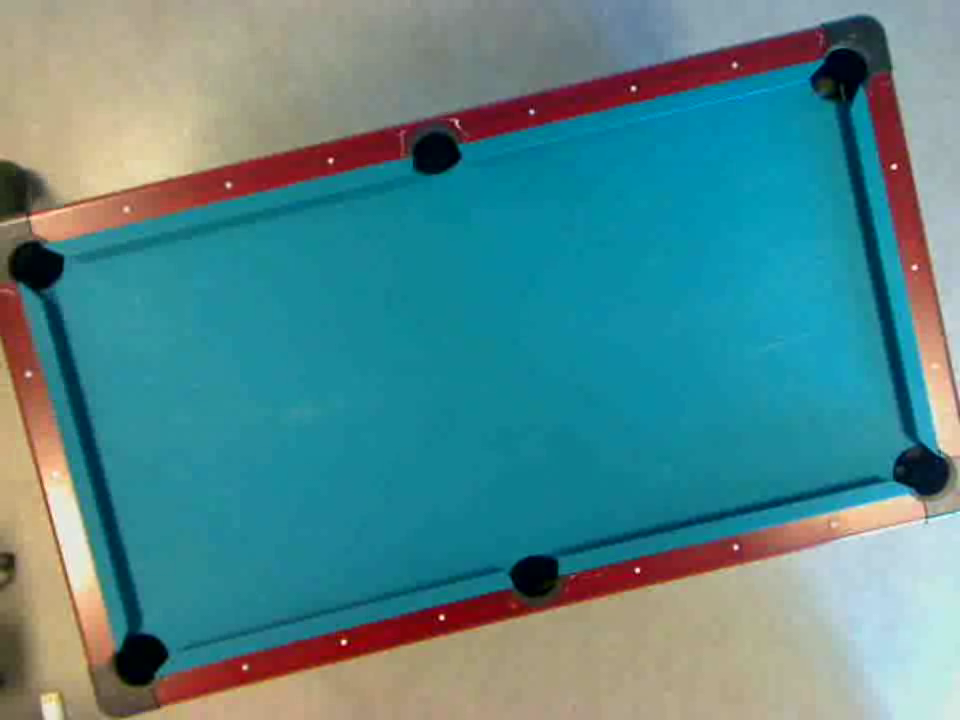
\includegraphics[width=0.4\textwidth]{images/montage_input}
}
\subfloat[Cloth ROI.]
{
	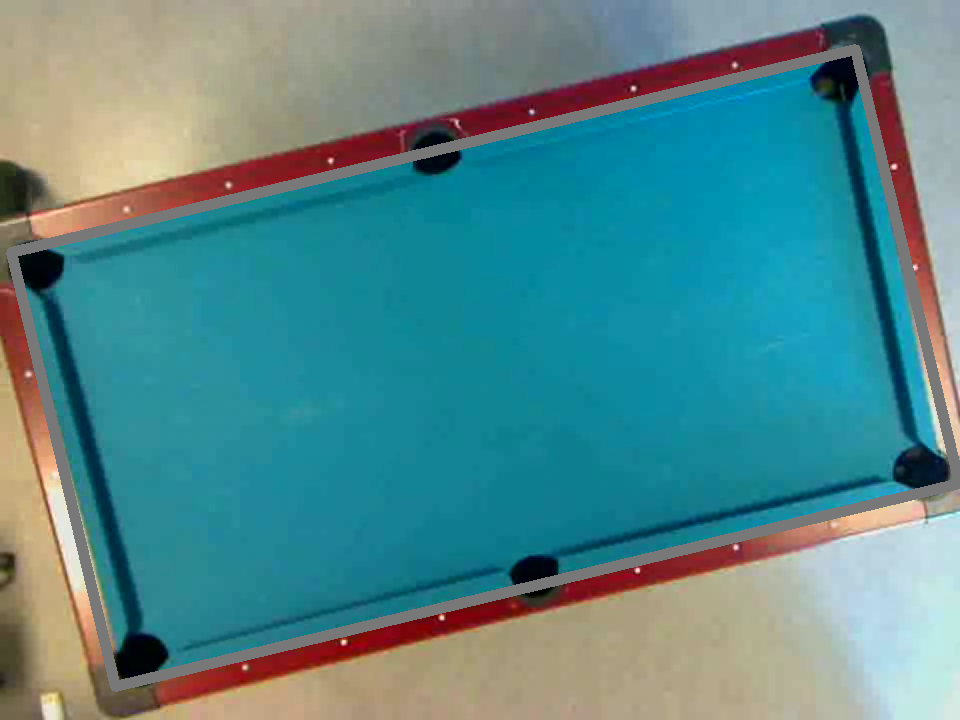
\includegraphics[width=0.4\textwidth]{images/montage_contour}
}
\\
\subfloat[Mask of cloth.]
{
	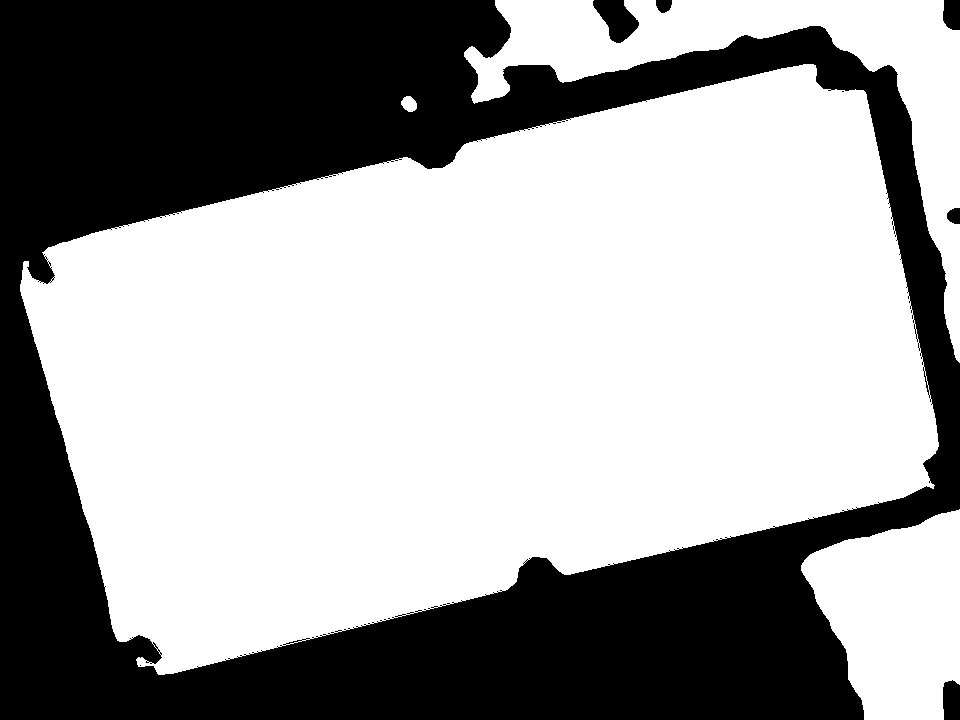
\includegraphics[width=0.4\textwidth]{images/montage_mask}
}
\subfloat[The output after rotating, cropping and setting mask.]
{
	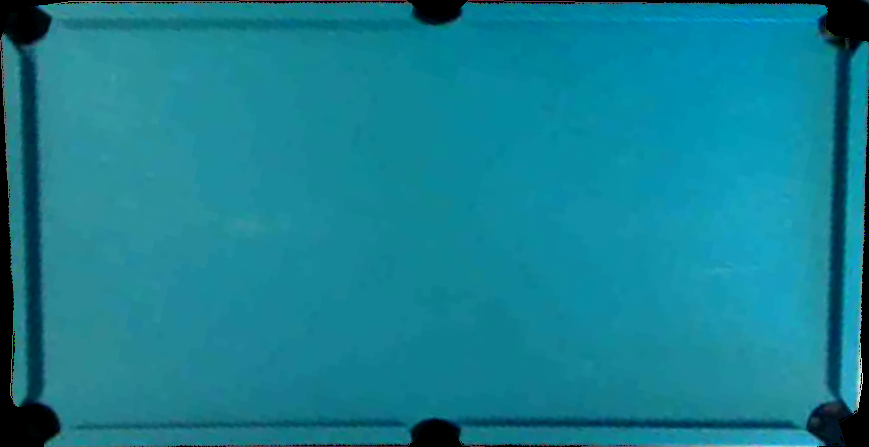
\includegraphics[width=0.4\textwidth]{images/montage_output}
}
\label{fig:tablelocateoutput}
\end{figure}

If the box for the non-rotated image is not found, then the angle is also not found. In this case the program will return a failure which indicates that the table is not found.